\documentclass[aspectratio=169,11pt]{beamer}
\usepackage[dvipsnames]{xcolor}
\usepackage{tikz}
\usepackage{mathtools}
\usepackage{multirow}
\usepackage{booktabs}
\usepackage{listings}

\lstdefinelanguage{julia}{
  morekeywords={using,end,function,return,for,in,if,else,elseif,while,let,do,begin,struct,abstract,mutable,type,const,global,local,where,break,continue,quote,true,false,nothing,Inf},
  morekeywords=[2]{ExaCore,ExaModel,Model,Optimizer,CUDABackend,ROCBackend,OneAPIBackend,MetalBackend,OpenCLBackend,CPU,CuArray},
  morekeywords=[3]{@add_var,@add_par,@add_obj,@add_con,@add_con!,@add_expr,@register_univariate,@register_bivariate,@variable,@constraint,@objective,@NLconstraint,@NLobjective},
  sensitive=true,
  morecomment=[l]{\#},
  morestring=[b]",
}
\definecolor{codecomment}{HTML}{006400} % dark green for code comments

\lstdefinestyle{darkrepl}{
  language={},
  basicstyle=\ttfamily\color{white}\tiny,
  backgroundcolor=\color{black},
  frame=single,
  frameround=tttt,
  framerule=0.4pt,
  rulecolor=\color{black},
  framesep=4pt,
  xleftmargin=4pt,
  xrightmargin=4pt,
  aboveskip=4pt,
  belowskip=4pt,
}
\lstset{
  language=julia,
  basicstyle=\ttfamily\scriptsize,
  keywordstyle=\color{mitred}\bfseries,
  keywordstyle=[2]\color{mitblue},
  keywordstyle=[3]\color{mitorange}\bfseries,
  commentstyle=\color{codecomment}\itshape,
  stringstyle=\color{mitdarkgray},
  showstringspaces=false,
  columns=fullflexible,
  keepspaces=true,
  breaklines=false,
  upquote=true,
  backgroundcolor=\color{mitlightgray!30},
  frame=single,
  frameround=tttt,
  framerule=0.4pt,
  rulecolor=\color{mitlightgray!50},
  framesep=4pt,
  xleftmargin=4pt,
  xrightmargin=4pt,
  aboveskip=4pt,
  belowskip=4pt,
}
\usepackage[style=authoryear-comp,url=false,date=year,doi=false,isbn=false,eprint=true,maxnames=1,minnames=1,backend=biber,natbib=true]{biblatex}

% ------------------------------------------------------------
% MIT COLOR PALETTE  (from MIT Brand Guidelines)
% ------------------------------------------------------------
\definecolor{mitred}{HTML}{A31F34}       % Primary MIT red
\definecolor{mitdarkgray}{HTML}{545454}  % Neutral dark gray
\definecolor{mitlightgray}{HTML}{C7C7C7} % Light gray
\definecolor{mitorange}{HTML}{D56F00}    % Secondary accent
\definecolor{mitblue}{HTML}{8A8BFF}      % Accent cool tone

% ------------------------------------------------------------
% APPLY TO TITLES
% ------------------------------------------------------------
\setbeamercolor{title}{fg=mitred}
\setbeamercolor{subtitle}{fg=mitdarkgray}
\setbeamercolor{frametitle}{fg=mitred}
\setbeamercolor{framesubtitle}{fg=mitdarkgray}
\setbeamercolor{section title}{fg=mitred}
\setbeamercolor{subsection title}{fg=mitdarkgray}

\setbeamercolor{structure}{fg=mitred}
\setbeamercolor{itemize item}{fg=mitred}
\setbeamercolor{itemize subitem}{fg=mitdarkgray}
\setbeamercolor{enumerate item}{fg=mitred}
\setbeamercolor{enumerate subitem}{fg=mitdarkgray}

\setbeamercolor{caption name}{fg=mitred}
\setbeamercolor{caption}{fg=mitdarkgray}

\setbeamertemplate{blocks}[rounded][shadow=false]
\setbeamercolor{block title}{fg=mitred,bg=mitorange!20}
\setbeamercolor{block body}{fg=mitdarkgray,bg=mitorange!20}
\setbeamercolor{block title alerted}{fg=mitred,bg=mitred!20}
\setbeamercolor{block body alerted}{fg=mitdarkgray,bg=mitred!20}
\setbeamercolor{block title example}{fg=mitred,bg=mitdarkgray!20}
\setbeamercolor{block body example}{fg=mitdarkgray,bg=mitdarkgray!20}

\setbeamercolor{alerted text}{fg=mitred}
\setbeamercolor{example text}{fg=mitblue}

\setbeamercolor{palette primary}{fg=white,bg=mitred}
\setbeamercolor{palette secondary}{fg=white,bg=mitdarkgray}
\setbeamercolor{palette tertiary}{fg=white,bg=mitdarkgray}
\setbeamercolor{palette quaternary}{fg=white,bg=mitdarkgray}

\setbeamercolor{separation line}{bg=mitlightgray}
\setbeamercolor{fine separation line}{bg=mitlightgray}

\hypersetup{
  colorlinks=true,
  linkcolor=mitred,
  urlcolor=mitred,
  citecolor=mitdarkgray
}

\setbeamersize{text margin left=0.5cm, text margin right=0.5cm}

\setbeamertemplate{navigation symbols}{}

\setbeamertemplate{footline}{%
  \leavevmode%
  \usebeamerfont{footline}
  \usebeamercolor[fg]{footline}
  \tiny
  \tikz[remember picture, overlay,xscale=0.875,transform shape]{
    \node[anchor=south] at (current page.south) {\insertshorttitle};
    \node[anchor=south west] at (current page.south west) {Sungho Shin--- \href{mailto:sushin@mit.edu}{\tt sushin@mit.edu}};
    \node[anchor=south east] at (current page.south east) {\insertframenumber/\inserttotalframenumber};
  }
}

\setbeamercolor{footline}{fg=mitdarkgray}
\setbeamerfont{footline}{size=\scriptsize}

\addbibresource{shin.bib}
\AtEveryCitekey{\clearfield{pages}}
\AtEveryCitekey{\clearfield{volume}}
\AtEveryCitekey{\clearfield{number}}
\AtEveryCitekey{\clearfield{primaryclass}}
\AtEveryCitekey{\clearfield{edition}}
\AtEveryCitekey{\clearfield{publisher}}
\AtEveryCitekey{\clearfield{series}}
\AtEveryCitekey{\clearfield{address}}
\DeclareNameAlias{default}{labelname}
\renewbibmacro{in:}{}

\newcommand{\refbr}[2][]{%
  \begin{tikzpicture}[remember picture, overlay,xscale=0.875,transform shape,inner sep=2pt]
    \node[anchor=south west,align=left,font=\tiny,color=mitdarkgray,text width=1.2\linewidth,yshift=10pt] at (current page.south west) {#1 #2};
  \end{tikzpicture}%
}

\newcommand{\joint}[2][]{%
  \begin{tikzpicture}[remember picture, overlay, xscale=0.875,transform shape,inner sep=2pt]
    \node[anchor=south west,align=left,font=\tiny,color=mitdarkgray] at (current page.south west) {#1 #2};
    \node[anchor=south east,align=left,font=\tiny,color=mitdarkgray] at (current page.south east) {\insertframenumber/\inserttotalframenumber};
  \end{tikzpicture}%
}

\graphicspath{{figs/}}

\title[Can ExaModels Power JuMP on GPUs?]{Can ExaModels Power JuMP on GPUs?}
\subtitle{Pattern-aware modeling and GPU-native automatic differentiation}
\author{
  Sungho Shin\\
  \url{shin.mit.edu}
}
\institute{
  Massachusetts Institute of Technology
}

\date{JuMP-dev 2026 \quad\textbar\quad Edinburgh}

\begin{document}

\frame{
  \thispagestyle{empty}
  \titlepage
  \begin{tikzpicture}[remember picture, overlay]
    \node[anchor=south, yshift=0.25cm] at (current page.south) {%
      \tiny
      \setlength{\tabcolsep}{2pt}%
      \begin{tabular}{cccccccccc}
        
\includegraphics[width=.42in]{shin.jpeg} &
        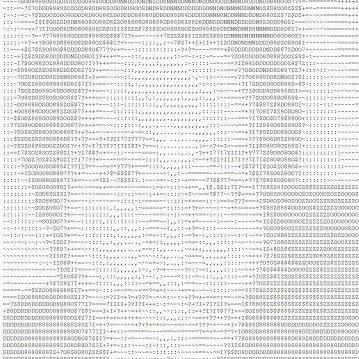
\includegraphics[width=.42in]{michel2323.jpeg} &
        
\includegraphics[width=.42in]{amontoison.jpeg} &
        
\includegraphics[width=.42in]{blegat.png} &
        
\includegraphics[width=.42in]{klamike.png} &
        
\includegraphics[width=.42in]{frapac.jpeg} &
        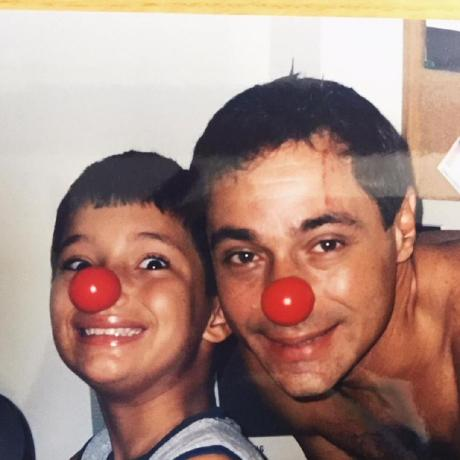
\includegraphics[width=.42in]{andrewrosemberg.jpeg} &
        
\includegraphics[width=.42in]{FHoltorf.png} &
        
\includegraphics[width=.42in]{jbcaillau.jpeg} &
        
\includegraphics[width=.42in]{hfytr.png} \\
        S. Shin & M. Schanen & A. Montoison & B. Legat & M. Klamkin &
        F. Pacaud & A. Rosemberg & F. Holtorf & J.-B. Caillau & Archim J \\
        {\color{mitdarkgray}\texttt{@sshin23}} &
        {\color{mitdarkgray}\texttt{@michel2323}} &
        {\color{mitdarkgray}\texttt{@amontoison}} &
        {\color{mitdarkgray}\texttt{@blegat}} &
        {\color{mitdarkgray}\texttt{@klamike}} &
        {\color{mitdarkgray}\texttt{@frapac}} &
        {\color{mitdarkgray}\texttt{@andrewrosemberg}} &
        {\color{mitdarkgray}\texttt{@FHoltorf}} &
        {\color{mitdarkgray}\texttt{@jbcaillau}} &
        {\color{mitdarkgray}\texttt{@hfytr}}
      \end{tabular}};
  \end{tikzpicture}
}

\setbeamertemplate{footline}[content]

% =============================================================
\section{What is ExaModels?}
% =============================================================
\begin{frame}[fragile]{What is ExaModels?}
  \begin{columns}[T]
    \begin{column}{.48\textwidth}
      \begin{itemize}\itemsep4pt
      \item \alert{Algebraic modeling system} in Julia, JuMP-inspired syntax.
      \item<2-> Builds on \texttt{NLPModels.jl} --- compatible with: \texttt{Ipopt}, \texttt{MadNLP}, \texttt{KNITRO}, \texttt{Uno}, \dots (essentially all JSO-style solvers)
      \item<3-> Ships with its own AD system --- $f(x),\; g(x),\; \nabla f(x),\; \nabla g(x),\; \nabla^2_{xx} L(x,\lambda)$
      \item<4-> \alert{\bfseries Killer feature}: \alert{GPU-compatible modeling} --- more on this later.
      \item<5-> \alert{\bfseries Design philosophy}: not optimized for ease-of-use, optimized for \alert{runtime performance}. Aim: the \alert{fastest modeling system} for building and running optimization solves.
      \end{itemize}
    \end{column}
    \begin{column}{.52\textwidth}
      \vspace{-1em}
      {\scriptsize\itshape Example: Goddard rocket --- maximize final altitude.\par}
      \lstinputlisting[basicstyle=\ttfamily\fontsize{6pt}{6pt}\selectfont]{code/03_what_is_snippet.jl}
    \end{column}
  \end{columns}
\end{frame}

% =============================================================
\section{Why GPU-native modeling, only for NLPs?}
% =============================================================
\begin{frame}{Why a GPU-compatible modeling language?}{LP / QP / DCP --- not strictly needed}
  \begin{columns}[T]
    \begin{column}{.58\textwidth}
      \begin{itemize}
      \item Canonical forms ($A, b, c$, ...) $\Rightarrow$ \alert{one-shot CPU$\to$GPU copy} of problem data
      \item Solver \alert{can iterate entirely on the device}
      \item Solution copied \alert{once back} to CPU
      \item Transfers can be an overhead, but the cost is \alert{amortized} over many solver iterations
      \item \alert{Existing GPU-native solvers} in this class already work this way: \texttt{CuClarabel}, \texttt{cuPDLP+}
      \item[]<2-> $\Rightarrow$ For LP / QP / DCP, a \alert{GPU-native modeling language may not add much value}
      \end{itemize}
    \end{column}
    \begin{column}{.40\textwidth}
      \centering
      \begin{tikzpicture}[every node/.style={font=\scriptsize, align=center},
                         baseline={(0,4.20)}]
        % Fixed bounding box --- identical across LP/QP and NLP slides
        \useasboundingbox (-2.2, -1.20) rectangle (2.2, 4.20);
        % --- Static elements (identical on the NLP slide) ---
        \node[anchor=south, inner sep=0] (cpu) at (0, 2.6)
          {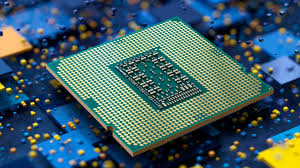
\includegraphics[width=2.0cm]{cpu_sungho.jpg}};
        \node[font=\bfseries, color=mitdarkgray] at (0, 3.92) {CPU};
        \node[anchor=north, inner sep=0] (gpu) at (0, 0.4)
          {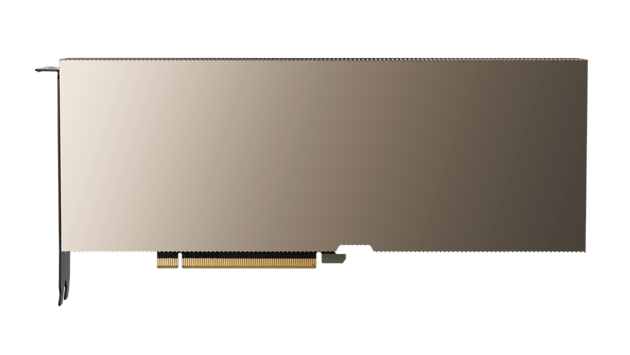
\includegraphics[width=2.0cm]{exa_a100_gpu.png}};
        \node[font=\bfseries, color=mitred] at (0, -1.00) {GPU};
        \filldraw[fill=mitorange!25, draw=mitorange, line width=0.6pt, rounded corners=2pt]
          (-1.7, 1.30) rectangle (1.7, 1.70);
        \node[font=\scriptsize\bfseries, color=mitorange!60!black] at (0, 1.50) {PCIe / SXM bus};
        % --- Arrows + labels (only this part differs from the NLP slide) ---
        \draw[->, very thick, mitred] (-0.55, 2.55) -- (-0.55, 0.45);
        \draw[->, very thick, mitred] (0.55, 0.45) -- (0.55, 2.55);
        \node[font=\tiny, color=mitdarkgray, anchor=east] at (-0.7, 2.15) {problem\\(once)};
        \node[font=\tiny, color=mitdarkgray, anchor=west] at (0.7, 0.85) {solution\\(once)};
      \end{tikzpicture}
    \end{column}
  \end{columns}
  \refbr{\fullcite{luCuPDLPFurtherEnhanced2025}}
\end{frame}

\begin{frame}{Why a GPU-compatible modeling language?}{NLP --- the picture is different}
  \begin{columns}[T]
    \begin{column}{.58\textwidth}
      \begin{itemize}\itemsep2pt
      \item Solver \alert{queries the modeling layer at every iteration} via \alert{callbacks} ---
        $f(x),\; g(x),\; \nabla f(x),\; \nabla g(x),\; \nabla^2_{xx} L(x,\lambda)$
      \item Each query depends on the current iterate---\alert{no one-shot transfer}
      \item Without GPU-native callbacks, every iteration pays a CPU$\leftrightarrow$GPU round-trip: \alert{significant per-iteration overhead, no amortization}
      \item<2-> JuMP today does \alert{not} emit GPU-native callbacks. Fine: modeling infrastructure stays on CPU, \alert{as long as the callbacks themselves run on the device}
      \end{itemize}
    \end{column}
    \begin{column}{.40\textwidth}
      \centering
      \begin{tikzpicture}[every node/.style={font=\scriptsize, align=center},
                         baseline={(0,4.20)}]
        % Identical bounding box + static elements as the LP/QP slide
        \useasboundingbox (-2.2, -1.20) rectangle (2.2, 4.20);
        \node[anchor=south, inner sep=0] (cpu) at (0, 2.6)
          {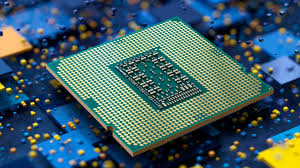
\includegraphics[width=2.0cm]{cpu_sungho.jpg}};
        \node[font=\bfseries, color=mitdarkgray] at (0, 3.92) {CPU};
        \node[anchor=north, inner sep=0] (gpu) at (0, 0.4)
          {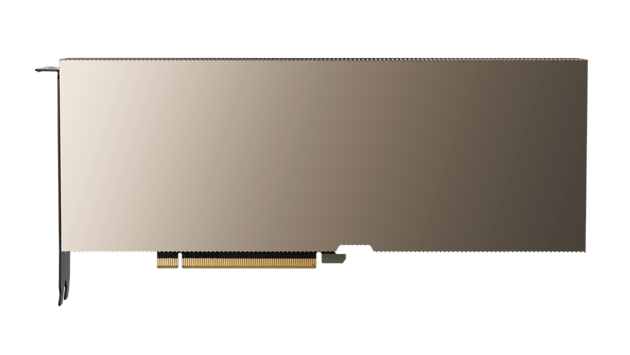
\includegraphics[width=2.0cm]{exa_a100_gpu.png}};
        \node[font=\bfseries, color=mitred] at (0, -1.00) {GPU};
        \filldraw[fill=mitorange!25, draw=mitorange, line width=0.6pt, rounded corners=2pt]
          (-1.7, 1.30) rectangle (1.7, 1.70);
        \node[font=\scriptsize\bfseries, color=mitorange!60!black] at (0, 1.50) {PCIe / SXM bus};
        % --- Arrows + iter labels (only this part differs from the LP/QP slide) ---
        \foreach \i in {0,1,2,3,4} {
          \pgfmathsetmacro{\x}{-0.80 + 0.40*\i}
          \draw[<->, thick, mitred] (\x, 2.55) -- (\x, 0.45);
        }
        \node[font=\scriptsize, color=mitdarkgray, anchor=east] at (-1.05, 2.15) {iter:};
        \foreach \i in {0,1,2,3,4} {
          \pgfmathsetmacro{\x}{-0.80 + 0.40*\i}
          \node[font=\tiny\bfseries, color=mitred, fill=white,
                inner sep=1pt, rounded corners=0.5pt] at (\x, 2.15) {\i};
        }
        \node[font=\tiny\bfseries, color=mitred, anchor=west, fill=white, inner sep=1pt]
          at (1.05, 2.15) {$\cdots$};
      \end{tikzpicture}
    \end{column}
  \end{columns}
\end{frame}

% =============================================================
\section{The ExaModels JuMP Interface}
% =============================================================
\begin{frame}[fragile]{The ExaModels JuMP Interface: Status Quo}
  \scriptsize
  \lstinputlisting{code/05_interface_snippet.jl}
  \medskip
  \normalsize
  \begin{itemize}
  \item Currently an \alert{experimental feature}: it works, but with \alert{big caveats} --- discussed in the next slides
  \end{itemize}
\end{frame}

\begin{frame}[fragile]{Model-build cost: JuMP route vs native ExaModels}
  \scriptsize
  \begin{columns}[T]
    \begin{column}{.49\textwidth}
      \alert{\bfseries JuMP route}
      \lstinputlisting{code/06_build_via_jump_snippet.jl}
      \smallskip
      \lstinputlisting[language={}, basicstyle=\ttfamily\scriptsize, backgroundcolor=\color{white}, frame=none, xleftmargin=0pt, xrightmargin=0pt, aboveskip=0pt, belowskip=0pt]{code/06_timing_jump.txt}
    \end{column}
    \begin{column}{.49\textwidth}
      \alert{\bfseries Native ExaModels}
      \lstinputlisting{code/06_build_native_snippet.jl}
      \smallskip
      \lstinputlisting[language={}, basicstyle=\ttfamily\scriptsize, backgroundcolor=\color{white}, frame=none, xleftmargin=0pt, xrightmargin=0pt, aboveskip=0pt, belowskip=0pt]{code/06_timing_native.txt}
    \end{column}
  \end{columns}
  \medskip
  \normalsize
  \begin{itemize}\itemsep1pt
  \item $\sim$\,\alert{7\,200$\times$ faster} build, $\sim$\,\alert{350$\times$ less memory}, $\sim$\,\alert{360{,}000$\times$ fewer allocations}
  \item<2-> The gap \alert{grows with $N$}
  \item<3-> ExaModels itself is faster than JuMP, but \alert{most of the overhead is in the JuMP $\to$ ExaModels conversion layer} (next slide)
  \end{itemize}
\end{frame}

% =============================================================
\section{Where the gap comes from}
% =============================================================
\begin{frame}[fragile]{Where the gap comes from: JuMP unrolls into a type-erased array}
  \scriptsize
  \lstinputlisting{code/07_typestable_jump.jl}
  \lstinputlisting[style=darkrepl]{code/07_typestable_jump_repl.txt}
  \medskip
  \normalsize
  \begin{itemize}\itemsep1pt
  \item JuMP \alert{unrolls the expression at construction} into a flat array of operators / operands
  \item<2-> The array is \texttt{Vector\{Any\}} --- the algebraic structure lives only in the \alert{runtime element types}, not in the array's static type
  \item<3-> Every conversion to ExaModels walks each node and pays \alert{type inference} per element $\Rightarrow$ that cost dominates the JuMP $\to$ ExaModels build
  \end{itemize}
\end{frame}

% =============================================================
\section{One remedy: hijack JuMP syntax (GenOpt.jl)}
% =============================================================
\begin{frame}[fragile]{One remedy: hijack the JuMP syntax (\texttt{GenOpt.jl} \citep{legatGenOptJl2025})}
  \begin{tikzpicture}[remember picture, overlay]
    \node[anchor=north east, xshift=-0.15cm, yshift=-0.15cm] at (current page.north east) {%
      \begin{tabular}{c}\scriptsize
        
\includegraphics[width=0.55in]{blegat.png}\\
        {\color{mitdarkgray}\texttt{@blegat}}
      \end{tabular}};
  \end{tikzpicture}%
\begin{lstlisting}
using GenOpt, JuMP, CUDA, MadNLP

@constraint(model, [i in 1:n], x[1,i] == x0[i],
    container = ParametrizedArray)                            # grouped constraint

@objective(model, Min,
    lazy_sum(0.5 * R[j] * u[i,j]^2 for i in 1:N, j in 1:p))   # grouped sum

set_optimizer(model, () -> GenOpt.ExaOptimizer(madnlp, CUDABackend()))
optimize!(model)
\end{lstlisting}
  \begin{itemize}
  \item Intercept JuMP's expression at construction time and route it to the ExaModels backend --- patterns survive intact, no scalar enumeration in the bridge.
  \item<2-> Minimal model rewrite: \texttt{container = ParametrizedArray} on \texttt{@constraint}, \texttt{lazy\_sum} on \texttt{@objective}
  \item<3-> A really cool proof-of-concept route --- I'm thinking about something else next.
  \end{itemize}
  \refbr{
    \fullcite{legatGenOptJl2025}
  }
\end{frame}

% =============================================================
\section{The expression tree is encoded in the type}
% =============================================================
\begin{frame}[fragile]{ExaModels: the type \emph{is} the tree}
  \begin{columns}[T]
    \begin{column}{.55\textwidth}
      \scriptsize
      \lstinputlisting{code/07_typestable_exa.jl}
      \lstinputlisting[style=darkrepl, belowskip=0pt]{code/07_typestable_exa_repl.txt}
    \end{column}
    \begin{column}{.43\textwidth}
      \centering
      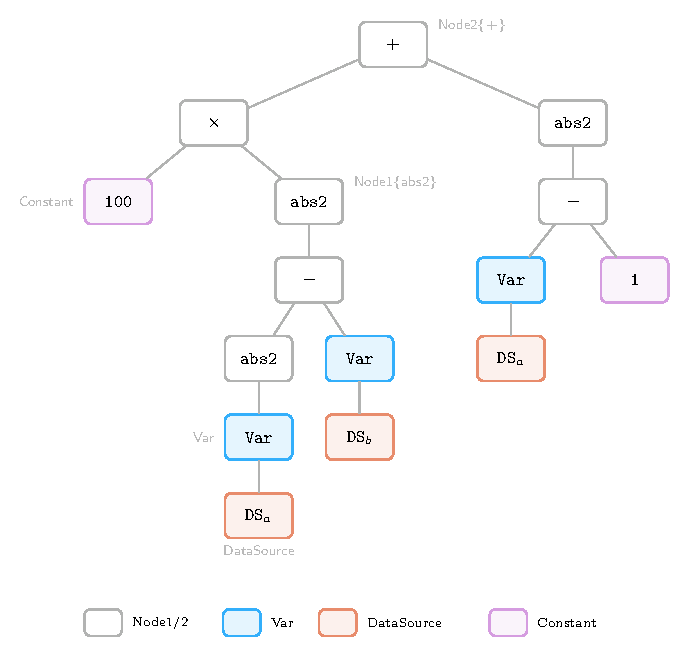
\includegraphics[height=.55\textheight]{exa_expression_tree.pdf}
    \end{column}
  \end{columns}
  \begin{itemize}\itemsep1pt
  \item \alert{ExaModels encodes the algebraic structure directly into the type system}
  \item Just by looking at the type, you can read the structure of the expression
  \item<2-> At compile time the structure is fully known $\Rightarrow$ \alert{model creation, AD, and evaluation are specialized for this algebraic expression}
  \end{itemize}
\end{frame}

\begin{frame}[fragile]{ExaModels: AD passes through the same typed tree}
  \begin{columns}[T]
    \begin{column}{.55\textwidth}
      \scriptsize
      \lstinputlisting{code/07_typestable_exa.jl}
      \lstinputlisting[style=darkrepl, belowskip=0pt]{code/07_typestable_exa_repl.txt}
    \end{column}
    \begin{column}{.43\textwidth}
      \centering
      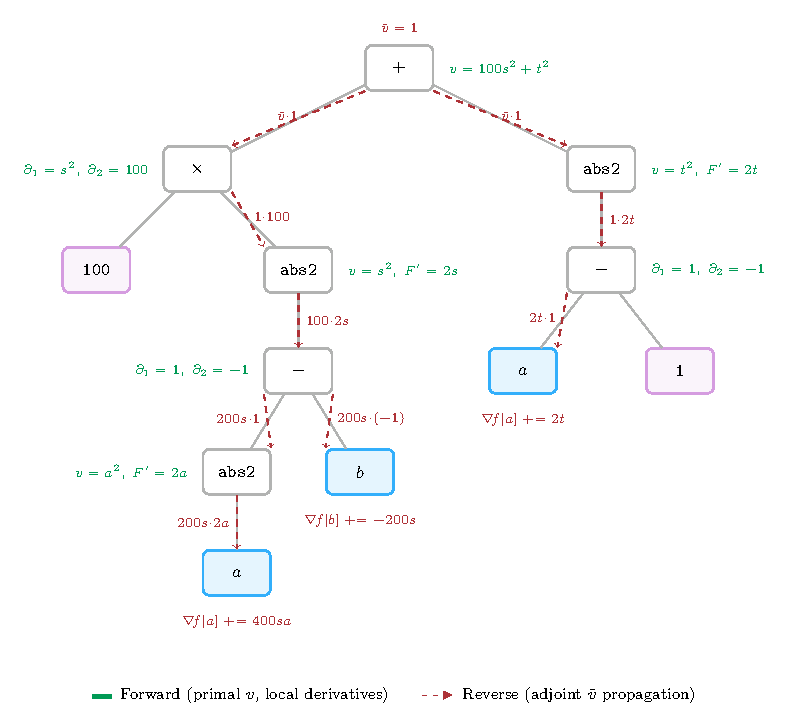
\includegraphics[height=.55\textheight]{exa_ad_passes.pdf}
    \end{column}
  \end{columns}
  \begin{itemize}\itemsep1pt
  \item Forward primals (green) and reverse adjoints (red) propagate through the \emph{same typed tree}
  \item<2-> \alert{Per-pattern sparsity is known at compile time} $\Rightarrow$ Jacobian + Hessian assembled in COO directly, \alert{no coloring round}, GPU-friendly
  \end{itemize}
\end{frame}

% =============================================================
\section{AOT compile: standalone binary}
% =============================================================
\begin{frame}[fragile]{Because the type knows everything: AOT compile to a standalone binary}
  \scriptsize
  \lstinputlisting{code/10_aot_snippet.jl}
  \lstinputlisting[style=darkrepl]{code/10_aot_build.txt}
  \smallskip
  \small
  \begin{itemize}\itemsep1pt
  \item A simple module: build a Rosenbrock model and call Ipopt
  \item \texttt{juliac --trim=safe} compiles it \alert{without the Julia runtime} --- same idea as a C shared library or executable
  \item<2-> Possible because the type is \alert{fully inferable at the modeling-function level}: the expression tree is fully known at compile time $\Rightarrow$ kernels for this NLP can be emitted AOT
  \end{itemize}
\end{frame}

% =============================================================
\section{Portability and performance}
% =============================================================
\begin{frame}{Portability and performance}{AD-callback speedup vs CPU-1T baseline, AC OPF (PGLIB-OPF)}
  \centering
  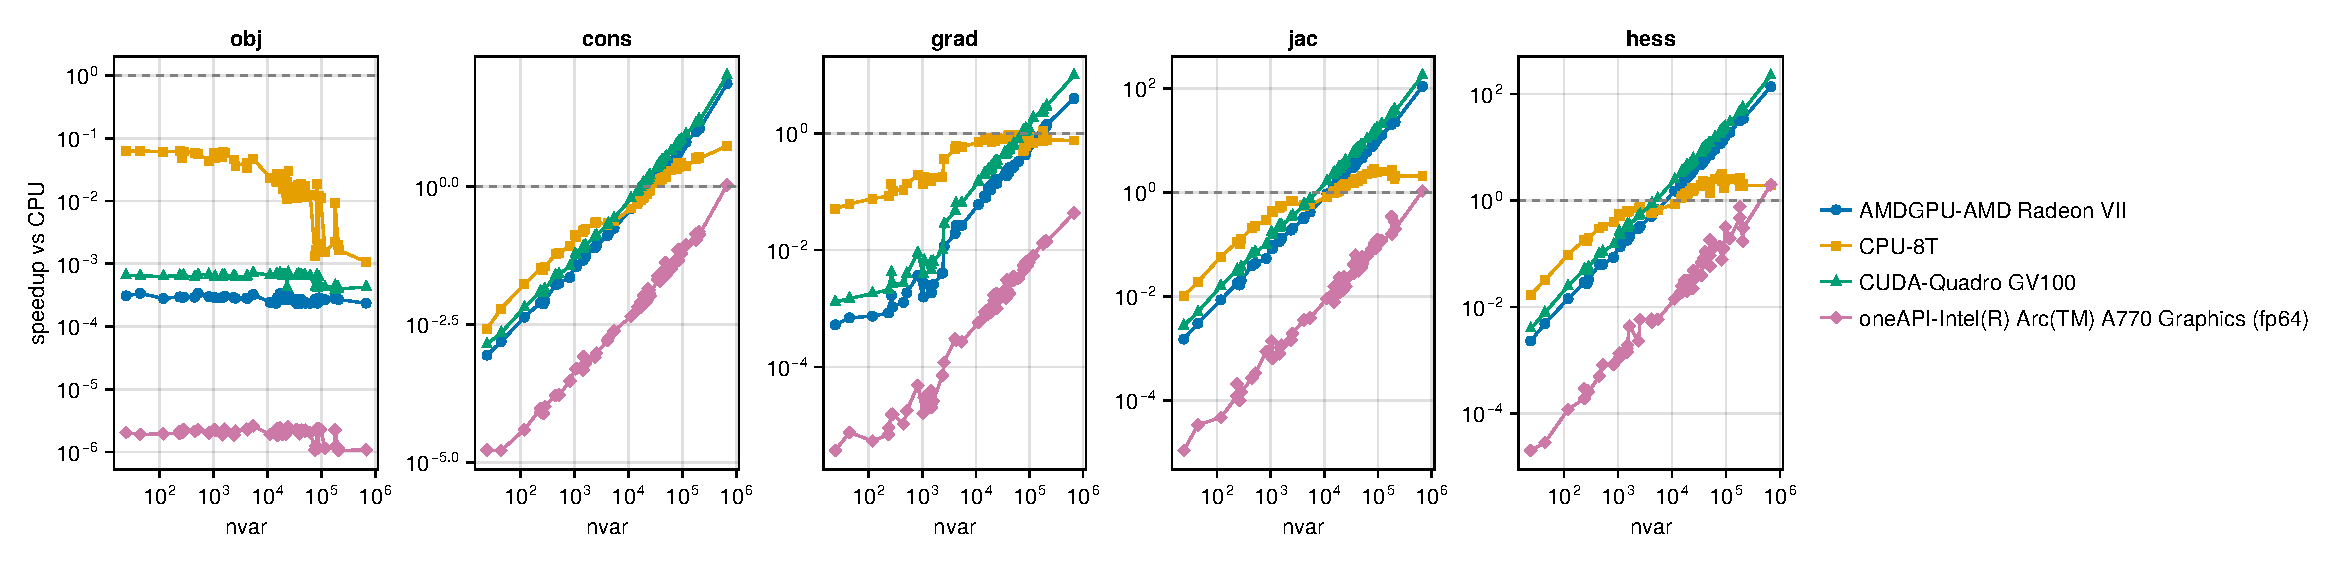
\includegraphics[width=.95\textwidth]{exa_backend_scaling.pdf}
  \begin{itemize}\itemsep1pt
  \item Tree complexity \alert{decoupled from the array level}: only \alert{data-level parallelism} is applied; per-data-point ops are scalar Julia, fully type-inferable
  \item<2-> Same model code runs on \texttt{CPU()}, \texttt{CUDABackend()}, \texttt{ROCBackend()}, \texttt{oneAPIBackend()}, \texttt{MetalBackend()} --- \alert{portable across GPU architectures}
  \item<3-> Jacobian / Hessian: CUDA, AMDGPU reach \alert{$>100\times$} at $n_{\text{var}} \sim 10^6$; \texttt{oneAPI} fp64 on Arc A770 is emulated $\Rightarrow$ hardware limit, not a software gap
  \end{itemize}
\end{frame}

\begin{frame}[fragile]{Trade-off: compile-once per algebraic pattern}
  \scriptsize Each new algebraic pattern triggers a fresh compile. Changing the expression --- even by one term --- counts as a new pattern.
  \medskip
  \begin{columns}[T]
    \begin{column}{.49\textwidth}
      \alert{\bfseries v1}
      \lstinputlisting{code/11_build_v1.jl}
    \end{column}
    \begin{column}{.49\textwidth}
      \alert{\bfseries v2 (added \texttt{sin(x[i])})}
      \lstinputlisting[moredelim={**[is][\color{mitred}\bfseries]{|}{|}}]{code/11_build_v2.jl}
    \end{column}
  \end{columns}
  \visible<2->{
  \medskip
  \lstinputlisting[style=darkrepl, basicstyle=\ttfamily\color{white}\scriptsize]{code/11_recompile_repl.txt}
  \scriptsize Identical re-builds hit the cache; the structural change in \texttt{v2} forces a fresh compile.
  }
\end{frame}

% =============================================================
\section{Alternative: ExaModels as a JuMP backend for GPU}
% =============================================================
\begin{frame}{Alternative: ExaModels as a JuMP backend for GPU acceleration}{Idea: a small bucket of fully-typed building blocks}
  \begin{itemize}\itemsep4pt
  \item Don't ask JuMP to be fully type-stable. Instead, give it a small \alert{bucket of building blocks} that are \alert{fully typed and concrete}
  \item<2-> $\sim$10 simple shapes of practical significance:
    \alert{linear}, \alert{quadratic}, \alert{generic polynomial},
    \alert{polynomial $\times\,\sin$}, \alert{polynomial $\times\,\exp$}, \dots
  \item<3-> JuMP authors against these blocks; ExaModels executes the conversion \alert{efficiently} over the bucket, with no per-element type inference
  \item<4-> Makes the JuMP $\to$ ExaModels conversion layer much easier to use --- without forcing JuMP's expression tree to be fully type-stable
  \end{itemize}
\end{frame}

% =============================================================
\section{Conclusion}
% =============================================================
\begin{frame}{Summary}
  \begin{center}
    \url{https://github.com/exanauts/ExaModels.jl}
  \end{center}
  \vspace{1em}
  \begin{itemize}
  \item ExaModels offers a \alert{SIMD abstraction} for NLPs---an alternative to vectorization that preserves indexed structure through (pattern, data iterator) pairs
  \item<2-> Type-stable parameterized expression tree + coloring-free sparse AD make \alert{GPU-native} derivative evaluation practical
  \item<3-> One model, six KA.jl backends, no code change
  \item<4-> Already the modeling layer for MadNLP's GPU-native interior-point methods
  \end{itemize}
  \refbr{\fullcite{pacaudCondensedspaceMethodsNonlinear2024}}
  \medskip
  \visible<5->{
    \begin{block}{Discussion --- and continuing this thread}
      \small We don't need to move all of JuMP onto the GPU. The win is \alert{GPU-native callbacks} eliminating the per-iteration round-trip. GenOpt.jl is a proof-of-concept; a slightly more type-stable JuMP expression tree (previous slide) would make the bridge cheap.\\[2pt]
      Continuing at \alert{SIAM Optimization 2026}: ``The State of ExaModels'' (MS369), \alert{Fri June 5, 11:10 BST}, 50 George Square G.03.
    \end{block}
  }
\end{frame}

\AtNextBibliography{\tiny}
\setbeamertemplate{bibliography item}{}
\begin{frame}{References}
  \tikz[text width=1.1\textwidth,xscale=.9,transform shape]{
    \node at (current page.center) {\printbibliography[heading=none]};
  }
\end{frame}

\end{document}

%%% Local Variables:
%%% mode: LaTeX
%%% TeX-master: t
%%% End:
